\chapter{Hardware Test} \label{app:hardware_test}
This appendix shows the results observed from the performed hardware test.

\section*{Servo motor rotation test} \label{app:servo_motor_test}
This section shows the observed values from the servo motor test. The test is performed according to the description in \secref{sec:servo_motor}. \tblref{table:app_motor_test} shows the raw rotation values collected from the test, as well as the difference between the two motors. 

\begin{table}[H]
	\centering
	\ra{1.3}
	\rowcolors{1}{Gray}{}
    \begin{tabular}{lccc}
    \hline  
    \rowcolor{DGray}
    \textbf{Power Level}~~~~~~~~~~~~ & Motor L(Degrees) & Motor R(Degrees) & Difference \\ \hline 
    100\%                  & 6,658                  & 6,666                & 0,12\% \\
    90\%                   & 5,823                  & 5,912                & 1,51\% \\
    80\%                   & 5,192                  & 5,262                & 1,33\% \\
    70\%                   & 4,495                  & 4,571                & 1,67\% \\
    60\%                   & 3,859                  & 3,923                & 1,64\% \\
    50\%                   & 3,145                  & 3,211                & 2,07\% \\
    40\%                   & 2,479                  & 2,551                & 2,86\% \\
    \hline  
    \end{tabular}
    \caption{\label{table:app_motor_test}Servo motor test of rotations.}
\end{table}

\newpage
\section*{Ultrasonic sensor distance test} \label{app:ultrasonic_sensor_test}
This section shows the observed values from the ultrasonic sensor distance test. \secref{sec:ultrasonic_sensor} describes the testing method. \tblref{table:app_ultrasonic_sensor_test} shows the observed sensor values, called value, and the actual distance. The difference between the values is also shown. 

\begin{table}[H]
	\centering
	\ra{1.3}
	\rowcolors{1}{Gray}{}
    \begin{tabular}{|lcc|lcc|}
    \hline  
    \rowcolor{DGray}
    \textbf{Actual distance} & \textbf{Value}  & \textbf{Difference} &\textbf{Actual distance} & \textbf{Value}  & \textbf{Difference}\\ \hline
    1 cm     & 8 cm     & 700\%  &    13 cm     & 16 cm     & 23\% \\
    2 cm     & 7 cm     & 250\%  &    14 cm     & 16 cm     & 14,2\% \\
    3 cm     & 6 cm     & 100\%  &    15 cm     & 17 cm     & 13,3\% \\
    4 cm     & 7 cm     & 75\%   &    20 cm     & 20 cm     & 0\% \\
    5 cm     & 7 cm     & 40\%   &    25 cm     & 25 cm     & 0\% \\
    6 cm     & 7 cm     & 16,6\% &    30 cm     & 32 cm     & 6,6\% \\
    7 cm     & 8 cm     & 14,2\% &    40 cm     & 41 cm     & 2,5\% \\
    8 cm     & 10 cm    & 25\%   &    50 cm     & 51 cm     & 2\% \\
    9 cm     & 11 cm    & 22,2\% &    100 cm    & 101 cm    & 1\% \\
    10 cm    & 13 cm    & 30\%   &    150 cm    & 150 cm    & 0\% \\
    11 cm    & 14 cm    & 27,2\% &    200 cm    & 255 cm    & 27,5\% \\
    12 cm    & 15 cm    & 25\%   &              &           &\\
    \hline 
    \end{tabular}
    \caption{\label{table:app_ultrasonic_sensor_test} Ultrasonic Sensor test at distances.}
\end{table}


\newpage
\section*{Ultrasonic rotation test graph} \label{app:sonar-test-graph}
This section shows the observations from the ultrasonic sensor rotation test plotted into a graph. Every time the values goes down, a new object has been spotted. There were placed five objects in this test.

The objects were placed at the following degrees:
\begin{description}
\item[Object 1] 0 degrees
\item[Object 2] 90 degrees
\item[Object 3] 180 degrees
\item[Object 4] 225 degrees
\item[Object 5] 270 degrees
\end{description}

\begin{figure}[H]
     \center{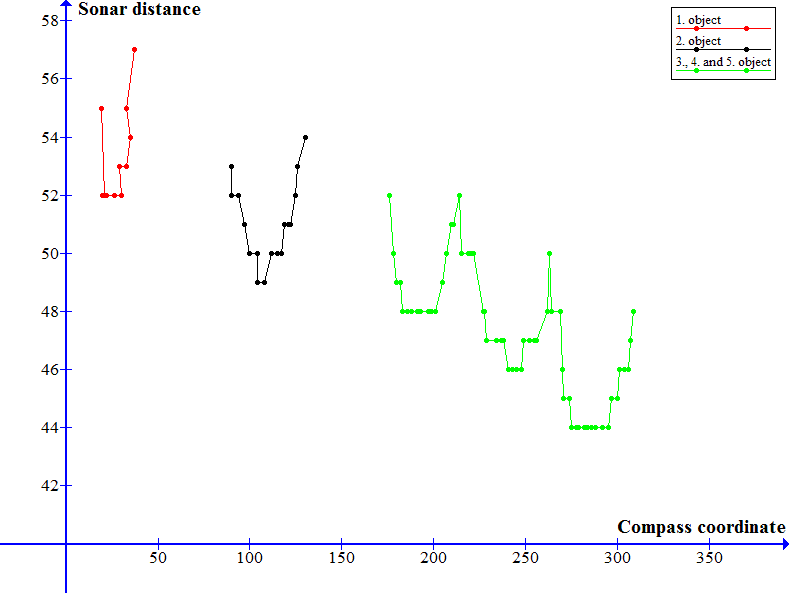
\includegraphics[width=\textwidth]
     {graphics/ObjectSpotting2.png}}
     \caption{\label{fig:sonar-test-graph} 360 degree test with ultrasonic sensor.}
\end{figure}

As seen in \figref{fig:sonar-test-graph}, if the objects are placed close together, the objects can not be distinguished from each other, resulting in object number 3., 4., and 5. counting as one big object. 







